%%%%%%%%%%%%%%%%%%%%%%%%%%%%%%%%%%%%%%%
% Wenneker Resume/CV
% LaTeX Template
% Version 1.1 (19/6/2016)
%
% This template has been downloaded from:
% http://www.LaTeXTemplates.com
%
% Original author:
% Frits Wenneker (http://www.howtotex.com) with extensive modifications by
% Vel (vel@LaTeXTemplates.com)
%
% License:
% CC BY-NC-SA 3.0 (http://creativecommons.org/licenses/by-nc-sa/3.0/
%
%%%%%%%%%%%%%%%%%%%%%%%%%%%%%%%%%%%%%%

%----------------------------------------------------------------------------------------
%	PACKAGES AND OTHER DOCUMENT CONFIGURATIONS
%----------------------------------------------------------------------------------------

\documentclass[a4paper,12pt]{memoir} % Font and paper size

%%%%%%%%%%%%%%%%%%%%%%%%%%%%%%%%%%%%%%%%%
% Wenneker Resume/CV
% Structure Specification File
% Version 1.1 (19/6/2016)
%
% This file has been downloaded from:
% http://www.LaTeXTemplates.com
%
% Original author:
% Frits Wenneker (http://www.howtotex.com) with extensive modifications by
% Vel (vel@latextemplates.com)
%
% License:
% CC BY-NC-SA 3.0 (http://creativecommons.org/licenses/by-nc-sa/3.0/)
%
%%%%%%%%%%%%%%%%%%%%%%%%%%%%%%%%%%%%%%%%%

%----------------------------------------------------------------------------------------
%	PACKAGES AND OTHER DOCUMENT CONFIGURATIONS
%----------------------------------------------------------------------------------------

\usepackage{XCharter} % Use the Bitstream Charter font
\usepackage[utf8]{inputenc} % Required for inputting international characters
\usepackage[T1]{fontenc} % Output font encoding for international characters

\usepackage[top=1cm,left=1cm,right=1cm,bottom=1cm]{geometry} % Modify margins

\usepackage{graphicx} % Required for figures

\usepackage{flowfram} % Required for the multi-column layout

\usepackage{url} % URLs

\usepackage[usenames,dvipsnames]{xcolor} % Required for custom colours

\usepackage{tikz} % Required for the horizontal rule

\usepackage{hyperref}

\usepackage{enumitem} % Required for modifying lists
\setlist{noitemsep,nolistsep} % Remove spacing within and around lists

\setlength{\columnsep}{\baselineskip} % Set the spacing between columns

% Define the left frame (sidebar)
\newflowframe{0.2\textwidth}{\textheight}{0pt}{0pt}[left]
\newlength{\LeftMainSep}
\setlength{\LeftMainSep}{0.2\textwidth}
\addtolength{\LeftMainSep}{1\columnsep}

% Small static frame for the vertical line
\newstaticframe{1.5pt}{\textheight}{\LeftMainSep}{0pt}

% Content of the static frame with the vertical line
\begin{staticcontents}{1}
\hfill
\tikz{\draw[loosely dotted,color=RoyalBlue,line width=1.5pt,yshift=0](0,0) -- (0,\textheight);}
\hfill\mbox{}
\end{staticcontents}

% Define the right frame (main body)
\addtolength{\LeftMainSep}{1.5pt}
\addtolength{\LeftMainSep}{1\columnsep}
\newflowframe{0.7\textwidth}{\textheight}{\LeftMainSep}{0pt}[main01]

\pagestyle{empty} % Disable all page numbering

\setlength{\parindent}{0pt} % Stop paragraph indentation

%----------------------------------------------------------------------------------------
%	NEW COMMANDS
%----------------------------------------------------------------------------------------

\newcommand{\userinformation}[1]{\renewcommand{\userinformation}{#1}} % Define a new command for the CV user's information that goes into the left column

\newcommand{\cvheading}[1]{{\Huge\bfseries\color{RoyalBlue} #1} \par\vspace{.6\baselineskip}} % New command for the CV heading
\newcommand{\cvsubheading}[1]{{\Large\bfseries #1} \bigbreak} % New command for the CV subheading

\newcommand{\Sep}{\vspace{1em}} % New command for the spacing between headings
\newcommand{\SmallSep}{\vspace{0.5em}} % New command for the spacing within headings

\newcommand{\aboutme}[2]{ % New command for the about me section
\textbf{\color{RoyalBlue} #1}~~#2\par\Sep
}

\newcommand{\CVSection}[1]{ % New command for the headings within sections
{\Large\textbf{#1}}\par
\SmallSep % Used for spacing
}

\newcommand{\CVItem}[2]{ % New command for the item descriptions
\textbf{\color{RoyalBlue} #1}\par
#2
\SmallSep % Used for spacing
}

\newcommand{\bluebullet}{\textcolor{RoyalBlue}{$\circ$}~~} % New command for the blue bullets
 % Include the file specifying document layout and packages

%----------------------------------------------------------------------------------------
%	NAME AND CONTACT INFORMATION
%----------------------------------------------------------------------------------------

\userinformation{ % Set the content that goes into the sidebar of each page
\begin{flushright}
% Comment out this figure block if you don't want a photo
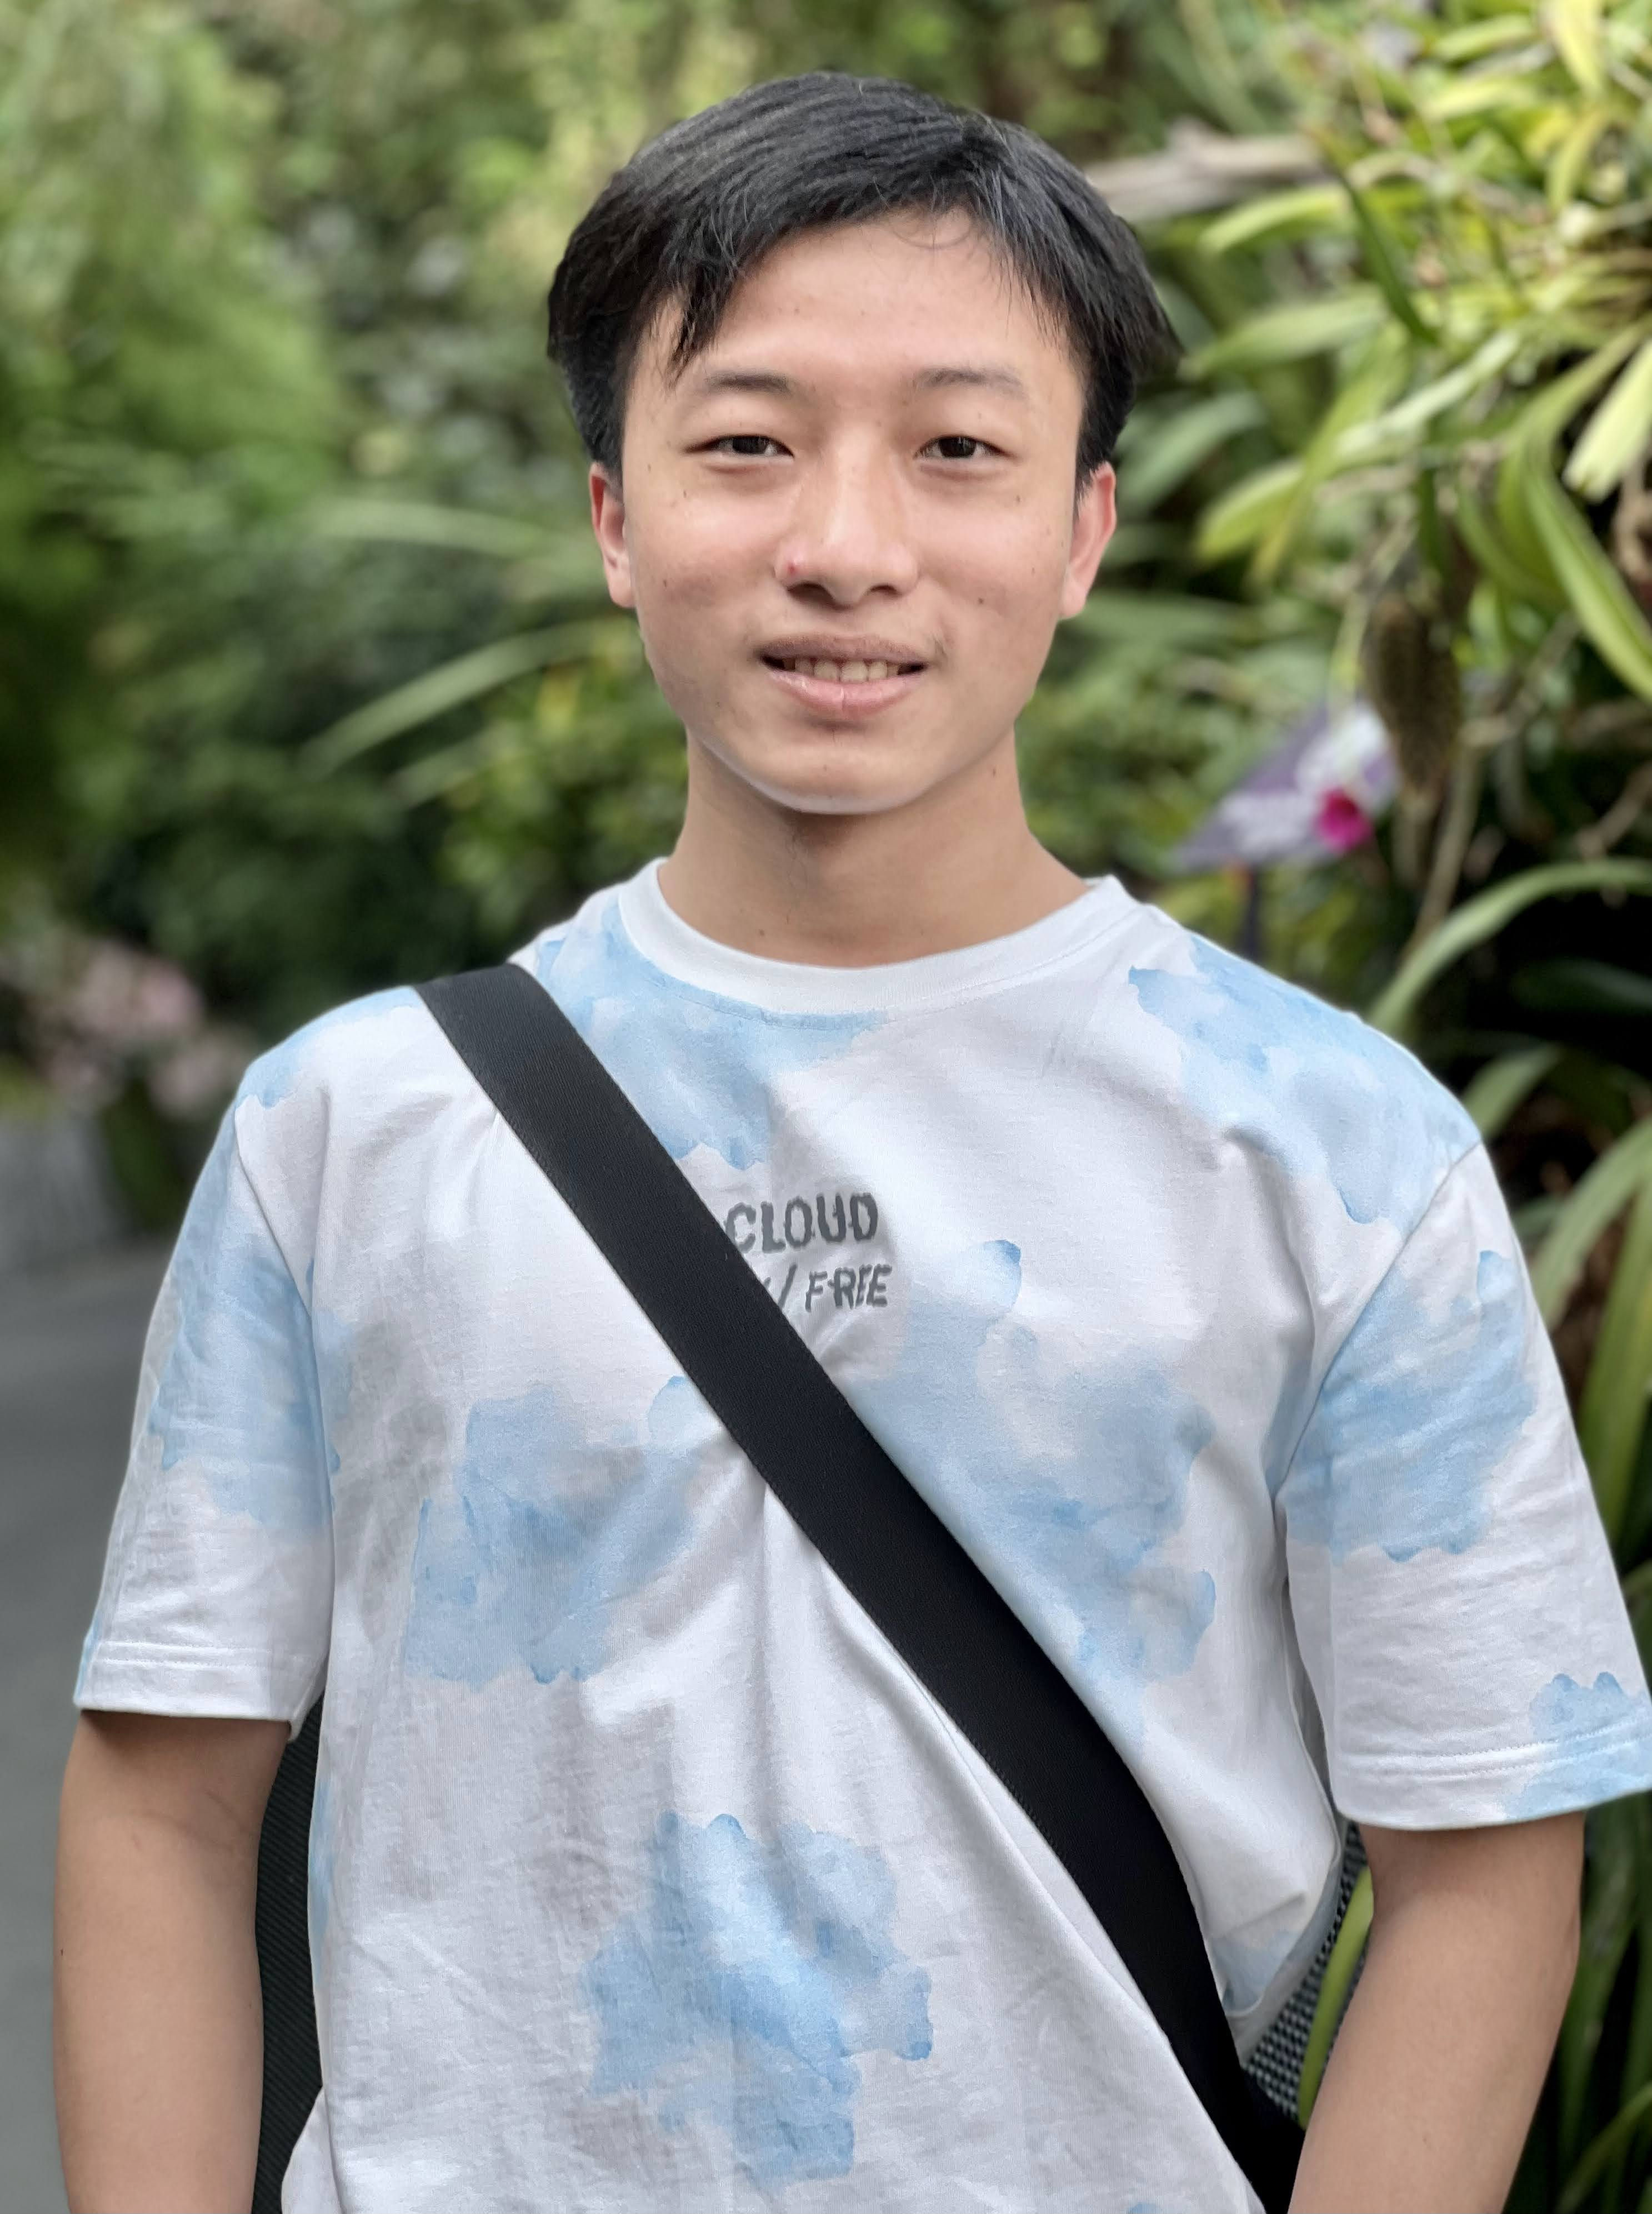
\includegraphics[width=0.6\columnwidth]{img/photo.jpg}\\[\baselineskip] % Your photo
\small % Smaller font size
Nguyen Minh Tien \\ % Your name
26-10-1999\\
\href{mailto:miti99@mail.com}{\em miti99@mail.com} \\ % Your email address
\href{https://miti99.gitlab.io/}{\em miti99.gitlab.io} \\ % Your URL
(+84) 869 156 149 \\ % Your phone number
\Sep % Some whitespace
\textbf{Address} \\
407 Tram Lac \\ % Address 1
My Hanh Bac \\ % Address 2
Duc Hoa, Long An \\ % Address 3
\vfill % Whitespace under this block to push it up under the photo
\end{flushright}
}

%----------------------------------------------------------------------------------------

\begin{document}

\userinformation % Print your information in the left column

\framebreak % End of the first column

%----------------------------------------------------------------------------------------
%	HEADING
%----------------------------------------------------------------------------------------

\cvheading{Nguyen Minh Tien} % Large heading - your name

\cvsubheading{Software Developer} % Subheading - your occupation/specialization

%----------------------------------------------------------------------------------------
%	ABOUT ME
%----------------------------------------------------------------------------------------

\aboutme{About Me}{A student who loves Linux and opensource softwares, using Archlinux and wants to customize it as much as possible.
\begin{itemize}
\item Gitlab: \href{https://gitlab.com/miti99/}{\em gitlab.com/miti99}
\item Github: \href{https://github.com/tien99/}{\em github.com/tien99}
\item Gmail: \href{mailto:minhtienit99@gmail.com}{\em minhtienit99@gmail.com}
\item School mail: \href{mailto:tien.nguyen.1999@hcmut.edu.vn}{\em tien.nguyen.1999@hcmut.edu.vn}
\item Facebook: \href{https://www.facebook.com/Tien.NM99/}{\em facebook.com/Tien.NM99}
\item Linkedin: \href{https://www.linkedin.com/in/miti99/}{\em linkedin.com/in/miti99}
\end{itemize}
}

%----------------------------------------------------------------------------------------
%	EDUCATION
%----------------------------------------------------------------------------------------

\CVSection{Education}

%------------------------------------------------

\CVItem{09/2017 - present, \href{https://hcmut.edu.vn/}{\em Ho Chi Minh City University of Technology}}{
  B.E. in Computer Science - \href{http://www.cse.hcmut.edu.vn/site/}{\em Faculty of Computer Science and Engineering}
}

%------------------------------------------------

%\Sep % Extra whitespace after the end of a major section

%----------------------------------------------------------------------------------------
%	EXPERIENCE
%----------------------------------------------------------------------------------------

%\CVSection{Experience}

%------------------------------------------------

%\CVItem{May 2013 - present, \textit{Software Engineer}, Google}{
%Detailed achievements:
%\begin{itemize}
%	\item Learned how to make amazing coffee
%	\item Finally determined the reason for \textsc{PC LOAD LETTER}:
%	\begin{itemize}
%		\item Paper jam
%		\item Software issues:
%		\begin{itemize}
%			\item Word not sending the correct data to printer
%			\item Windows trying to print in letter format
%		\end{itemize}
%		\item Coffee spilled inside printer
%	\end{itemize}
%	\item Broke the office record for number of kitten pictures in cubicle
%	\item Learned how to make more amazing coffee on a new machine
%	\item Mastered the art of filing accurate TPS reports
%\end{itemize}
%}

%------------------------------------------------

%\CVItem{Jan 2008 - Oct 2012, \textit{Computer Repair Specialist}, Buy More}{Worked in the Nerd Herd and helped to solve computer problems by asking customers to turn their computers off and on again.}

%------------------------------------------------

%\Sep % Extra whitespace after the end of a major section

%----------------------------------------------------------------------------------------
%	COMMUNICATION SKILLS
%----------------------------------------------------------------------------------------

%\CVSection{Communication Skills}

%------------------------------------------------

%\CVItem{2015, \textit{Oral Presentation}, California Business Conference}{Presented research I conducted for my Masters of Engineering degree.}

%------------------------------------------------

%\CVItem{2014, \textit{Poster}, Annual Business Conference (Oregon)}{As part of the course work for BUS320, I created a poster analyzing several local businesses and presented this at a conference.}

%------------------------------------------------

\Sep % Extra whitespace after the end of a major section

%----------------------------------------------------------------------------------------
%	SKILLS
%----------------------------------------------------------------------------------------

\CVSection{Technical Skills}

%------------------------------------------------

\CVItem{Programming Languages}
{\begin{tabular}{p{0.2\textwidth} p{0.2\textwidth} p{0.2\textwidth}}
\bluebullet C/C++ &  \bluebullet Javascript & \bluebullet LaTeX\\
\bluebullet PHP &  \bluebullet SQL & \bluebullet Go\\
\end{tabular}}

\CVItem{Databases}{
  \begin{tabular}{p{0.2\textwidth} p{0.2\textwidth} p{0.2\textwidth}}
  \bluebullet MySQL & \bluebullet MongoDB&\\
  \end{tabular}
}

\CVItem{Frameworks, Libraries}{
  \begin{tabular}{p{0.2\textwidth} p{0.2\textwidth} p{0.2\textwidth}}
    \bluebullet NodeJS &&\\
    \end{tabular}
}

%------------------------------------------------

\CVItem{Computer Softwares}
{\begin{tabular}{p{0.2\textwidth} p{0.2\textwidth} p{0.2\textwidth}}
\bluebullet VS Code & \bluebullet Qt Creator & \bluebullet Git\\
\end{tabular}}

%------------------------------------------------

%\Sep % Extra whitespace after the end of a major section

%----------------------------------------------------------------------------------------
%	NEW PAGE DELIMITER
%	Place this block wherever you would like the content of your CV to go onto the next page
%----------------------------------------------------------------------------------------

%\clearpage % Start a new page

%\userinformation % Print your information in the left column

%\framebreak % End of the first column

%----------------------------------------------------------------------------------------
%	AWARDS
%----------------------------------------------------------------------------------------

%\CVSection{Awards}

%------------------------------------------------

%\CVItem{2010, \textit{Postgraduate Scholarship}, Cornell University}{Awarded to the top student in their final year of a Bachelors degree.}

%------------------------------------------------

\Sep

\CVSection{Projects}

\CVItem{2018 - 2019, \textit{Some personal Facebook tools}}{
  \begin{itemize}
  \item Facebook chatbot for my profile using Python, deployed on \href{https://heroku.com/}{\em Heroku}.
  \item Facebook chatbot for my team's fanpage (\href{https://www.facebook.com/bkfcduchoalongan/}{\em BKFC - THPT Duc Hoa}) using NodeJS. (deprecated - replaced with our website).
  \item Facebook messages counting tools using Python for local tool, NodeJS for online tool: count the number of messages users have chatted with their friends.
  \end{itemize}
}

\CVItem{2020 - present, {Static websites with Hugo}}{
  \begin{itemize}
  \item My blog on Gitlab Pages - \href{https://miti99.gitlab.io/}{\em miti99.gitlab.io} using \href{https://gohugo.io/}{\em Hugo}. I use it to replace my old \href{https://miti99.code.blog}{\em WordPress blog}.
  \item My team's website \href{https://bkfc-thptduchoa.netlify.app/}{\em bkfc-thptduchoa.netlify.app} using the same tools as my blog's with some tweaks for posting contents:
    \begin{itemize}
    \item Allow post with LaTex to present Math equations on posts.
    \item Allow students to comment to our posts if they have questions.
    \end{itemize}
  \end{itemize}
}

\Sep % Extra whitespace after the end of a major section

%----------------------------------------------------------------------------------------
%	INTERESTS
%----------------------------------------------------------------------------------------

\CVSection{Interests}

%------------------------------------------------

\CVItem{Professional}{Facebook chatbot, static web design, blogging, software design}

%------------------------------------------------

\CVItem{Personal}{Playing chess, rubik, reading light novel-, manga}

%------------------------------------------------

\Sep % Extra whitespace after the end of a major section

%----------------------------------------------------------------------------------------

\end{document}
